\documentclass[11pt]{article}

% Required packages for arXiv submission
\usepackage[utf8]{inputenc}
\usepackage[T1]{fontenc}
\usepackage{amsmath,amsfonts,amssymb,amsthm}
\usepackage{graphicx}
\usepackage{hyperref}
\usepackage{url}
\usepackage{booktabs}
\usepackage{algorithm}
\usepackage{algorithmic}
\usepackage[margin=1in]{geometry}

% Hyperref setup
\hypersetup{
    colorlinks=true,
    linkcolor=blue,
    citecolor=red,
    urlcolor=blue,
}

% Title and author information
\title{Exploring Transformer Architectures for Time Series Forecasting: An Empirical Study of Causal vs. Bidirectional Attention}

\author{Chao Ma\\
Independent Researcher\\
\texttt{ickma2311@gmail.com}
}

\date{}

\begin{document}

\maketitle

\begin{abstract}
Time series forecasting has seen significant advances with transformer architectures, yet questions remain about their true competitiveness compared to traditional statistical methods. We provide a comprehensive empirical comparison of transformer variants (standard Transformer, Large Transformer, decoder-only, LSTM) against traditional methods (ARIMA, Prophet, XGBoost, Linear) using rigorous moving-window validation. Unlike prior work based solely on static train/test splits, our evaluation uses rolling moving-window protocol across both synthetic and real-world datasets. Results reveal that standard Transformer architecture achieves remarkable performance, ranking \\#2 globally with only 2.1\\% performance gap behind ARIMA (4.029 vs 3.947 MAE). This challenges previous conclusions about neural network limitations and demonstrates that evaluation methodology fundamentally determines research conclusions. We show that simpler transformer architectures consistently outperform complex ones, and provide evidence-based guidance for practitioners choosing between neural and traditional forecasting methods.
\end{abstract}

\noindent\textbf{Keywords:} Time series forecasting, transformer architecture, causal attention, autoregressive modeling, neural networks

\section{Introduction}

Time series forecasting remains a fundamental challenge across numerous domains, from financial markets and supply chain management to weather prediction and energy consumption planning. While traditional statistical methods like ARIMA and exponential smoothing have dominated the field for decades, recent advances in deep learning have introduced powerful alternatives, particularly transformer architectures originally designed for natural language processing.

The transformer architecture's success in sequence modeling has naturally led to its adoption in time series forecasting. However, most existing approaches directly adapt encoder-only transformers with bidirectional attention, which can access future information during training—a fundamental violation of temporal causality in forecasting tasks. This architectural choice may limit the model's ability to learn proper temporal dependencies and generalize to real-world forecasting scenarios.

\subsection{Problem Statement}

Current transformer-based time series forecasting methods face several key limitations:

\begin{enumerate}
\item \textbf{Temporal causality violation}: Encoder-only architectures with bidirectional attention can ``see'' future values during training
\item \textbf{Parameter inefficiency}: Larger models don't necessarily yield better performance for time series
\item \textbf{Limited empirical comparison}: Few studies comprehensively compare neural approaches against domain-specific traditional methods
\item \textbf{Architecture design gaps}: Insufficient exploration of decoder-only architectures for time series
\end{enumerate}

\subsection{Contributions}

This paper makes the following key contributions:

\begin{enumerate}
\item \textbf{Novel Architecture}: We introduce a decoder-only transformer with causal attention specifically designed for time series forecasting
\item \textbf{Comprehensive Evaluation}: We provide an extensive empirical comparison across 8 methods and 60 time series with diverse patterns
\item \textbf{Performance Breakthrough}: We demonstrate that decoder-only transformers achieve state-of-the-art results while being parameter-efficient
\item \textbf{Architectural Insights}: We show that proper attention mechanisms matter more than model size for time series forecasting
\item \textbf{Practical Guidelines}: We provide actionable recommendations for practitioners choosing forecasting methods
\end{enumerate}

\section{Related Work}

\subsection{Traditional Time Series Forecasting}

Classical time series forecasting has been dominated by statistical methods. \textbf{ARIMA} (AutoRegressive Integrated Moving Average) models excel at capturing autoregressive patterns and remain the gold standard for stationary time series~\cite{box1976time}. \textbf{Exponential smoothing} methods and \textbf{Prophet}~\cite{taylor2018forecasting} have proven effective for business forecasting with clear trend and seasonal patterns.

More recently, \textbf{gradient boosting} methods like XGBoost have been applied to time series by treating forecasting as a supervised learning problem with engineered temporal features~\cite{chen2016xgboost}. These methods bridge the gap between traditional statistics and modern machine learning.

\subsection{Neural Network Approaches}

\textbf{Recurrent Neural Networks} (RNNs) and \textbf{Long Short-Term Memory} (LSTM) networks were among the first successful neural approaches to time series forecasting~\cite{hochreiter1997long}. However, they suffer from vanishing gradients and limited ability to capture long-range dependencies.

\textbf{Convolutional Neural Networks} have also been explored for time series, treating sequences as 1D signals~\cite{bai2018empirical}. While effective for some applications, they lack the dynamic attention mechanisms crucial for complex temporal patterns.

\subsection{Transformer-Based Forecasting}

The introduction of transformers to time series forecasting has shown promising results~\cite{vaswani2017attention}. \textbf{Informer}~\cite{zhou2021informer} addresses the quadratic complexity of attention for long sequences. \textbf{Autoformer}~\cite{wu2021autoformer} introduces decomposition-based attention mechanisms. \textbf{FEDformer}~\cite{zhou2022fedformer} employs Fourier transforms for frequency domain modeling.

However, most existing approaches use encoder-only architectures with bidirectional attention, potentially compromising temporal causality. Recent work like \textbf{PatchTST}~\cite{nie2023time} and \textbf{iTransformer}~\cite{liu2024itransformer} have shown promising results, while \textbf{TEMPO}~\cite{chen2024tempo} explores GPT-style architectures for time series. Despite these advances, questions remain about transformer effectiveness for time series~\cite{zeng2023transformers}. Our work addresses fundamental limitations by introducing decoder-only architectures with proper causal masking, building on comprehensive surveys of the field~\cite{wen2022transformers}.

\section{Methodology}

\subsection{Experimental Design}

We conduct a comprehensive empirical study comparing eight forecasting methods across three categories:

\textbf{Traditional Methods:}
\begin{itemize}
\item ARIMA with automatic order selection
\item Prophet with trend and seasonality decomposition  
\item Linear baseline using recent value extrapolation
\item XGBoost with engineered temporal features
\end{itemize}

\textbf{Neural Network Methods:}
\begin{itemize}
\item Standard Transformer (565K parameters, encoder-only)
\item Large Transformer (4.85M parameters, encoder-only)
\item Decoder-Only Transformer (136K parameters, causal attention)
\item LSTM baseline (51K parameters)
\end{itemize}

\subsection{Dataset Generation}

We generate three synthetic datasets to control for pattern complexity and ensure reproducible evaluation:

\begin{enumerate}
\item \textbf{Trend-Seasonal (20 series, 200 points each)}: Linear trends with seasonal patterns mimicking business data
\item \textbf{Multi-Seasonal (20 series, 300 points each)}: Overlapping seasonal cycles of different frequencies
\item \textbf{Random Walk (20 series, 150 points each)}: Stochastic processes with unpredictable autoregressive behavior
\end{enumerate}

Each dataset contains 20 time series with known ground truth patterns, totaling 60 series and approximately 13,000 data points.

\subsection{Decoder-Only Transformer Architecture}

Our proposed decoder-only transformer differs fundamentally from existing encoder-only approaches:

\subsubsection{Architecture Components}

\begin{align}
\text{Input Sequence: } &[x_1, x_2, \ldots, x_t] \nonumber\\
&\downarrow \nonumber\\
\text{Input Projection: } &\text{Linear}(1 \to d_{\text{model}}) \nonumber\\
&\downarrow \nonumber\\
\text{Positional Encoding: } &\text{Sinusoidal position embeddings} \nonumber\\
&\downarrow \nonumber\\
\text{Decoder Layers: } &\text{Self-attention with causal masking} \nonumber\\
&\downarrow \nonumber\\
\text{Output Projection: } &\text{Linear}(d_{\text{model}} \to 1) \nonumber\\
&\downarrow \nonumber\\
\text{Next Value: } &y_{t+1} \nonumber
\end{align}

\subsubsection{Causal Attention Mechanism}

Unlike encoder-only transformers that use bidirectional attention, our decoder-only architecture employs causal masking:

\begin{algorithmic}
\STATE \textbf{function} \textsc{GenerateCausalMask}(seq\_len)
\STATE mask $\leftarrow$ upper\_triangular\_matrix(seq\_len, seq\_len, diagonal=1)
\STATE \textbf{return} mask.bool()
\end{algorithmic}

This ensures that predictions at time step $t$ only depend on information from steps $1, 2, \ldots, t-1$, maintaining strict temporal causality.

\subsubsection{Autoregressive Generation}

During inference, the model generates forecasts autoregressively:
\begin{enumerate}
\item \textbf{Single-step prediction}: $\hat{y}_{t+1} = f(\mathbf{x}_{1:t})$
\item \textbf{Sequence update}: $\mathbf{x}_{2:t+1} = [\mathbf{x}_{2:t}, \hat{y}_{t+1}]$
\item \textbf{Recursive generation}: Repeat for desired forecast horizon
\end{enumerate}

This approach contrasts with encoder-only models that predict entire future sequences simultaneously.

\subsection{Training Procedure}

All neural models are trained using:
\begin{itemize}
\item \textbf{Loss function}: Mean Squared Error (MSE)
\item \textbf{Optimizer}: Adam~\cite{kingma2014adam} with learning rate 0.001
\item \textbf{Training epochs}: 20 for transformers, 50 for LSTM
\item \textbf{Batch size}: 32 (16 for large transformer)
\item \textbf{Sequence length}: 50 steps for input
\item \textbf{Forecast horizon}: 10 steps
\end{itemize}

\textbf{Teacher forcing} is employed during decoder-only training, where ground truth values are used as inputs rather than model predictions, ensuring stable training. All implementations use PyTorch~\cite{paszke2019pytorch} for neural networks and scikit-learn~\cite{pedregosa2011scikit} for traditional methods.

\subsection{Transformer Architectures}

We compare encoder-only and decoder-only variants:
\begin{itemize}
    \item \textbf{Encoder-only (Transformer, LargeTransformer)}: input projection to $d_{model}$, sinusoidal positional encoding, $L$ TransformerEncoder layers (multi-head self-attention with $h$ heads and feed-forward of size $4\,d_{model}$), and a prediction head mapping the last time step to a multi-step horizon.
    \item \textbf{Decoder-only (causal)}: masked self-attention stack implemented via TransformerEncoder with an upper-triangular causal mask (no cross-attention/memory), trained with teacher forcing to predict the next step and rolled out autoregressively for multi-step forecasts.
\end{itemize}

\subsection{Datasets}

We evaluate on five datasets spanning synthetic and real-world settings:
\begin{itemize}
    \item \textbf{Synthetic} (controlled): trend-seasonal (20 series, length~\textasciitilde200), multi-seasonal (20, length~\textasciitilde300), random walk (20, length~\textasciitilde150), generated by our script with fixed seeds.
    \item \textbf{Retail sales} (real-world style): 20 daily series with realistic trends, weekly/annual seasonality, and holiday effects.
    \item \textbf{Energy consumption} (real-world style): 10 hourly series with daily/weekly/annual cycles and weather noise.
\end{itemize}

Each dataset is saved as a metadata CSV (series id, lengths) and NPZ values file for reproducibility.

\subsection{Evaluation Protocol (Moving-Window)}

Our primary evaluation uses rolling-origin moving-window validation to measure temporal generalization. For each series, we select a window of size $W = \min(\text{window\_size}, \lfloor \frac{\text{len(series)}}{3} \rfloor)$ and slide it to obtain $N = \min(\text{max\_windows}, \text{len(series)} - W - 1)$ windows. At each window:
\begin{enumerate}
    \item Fit the model on the window data
    \item Predict the next step
    \item Collect (prediction, target)
\end{enumerate}
We report Mean Absolute Error (MAE) and Root Mean Squared Error (RMSE) aggregated across windows (per series) and then averaged across series.

\section{Results (Moving-Window Evaluation)}

Our comprehensive moving-window evaluation reveals performance differences across methods and model types. Figure~\ref{fig:overall_performance} shows overall rankings aggregated across windows and series.

\begin{figure}[h]
\centering
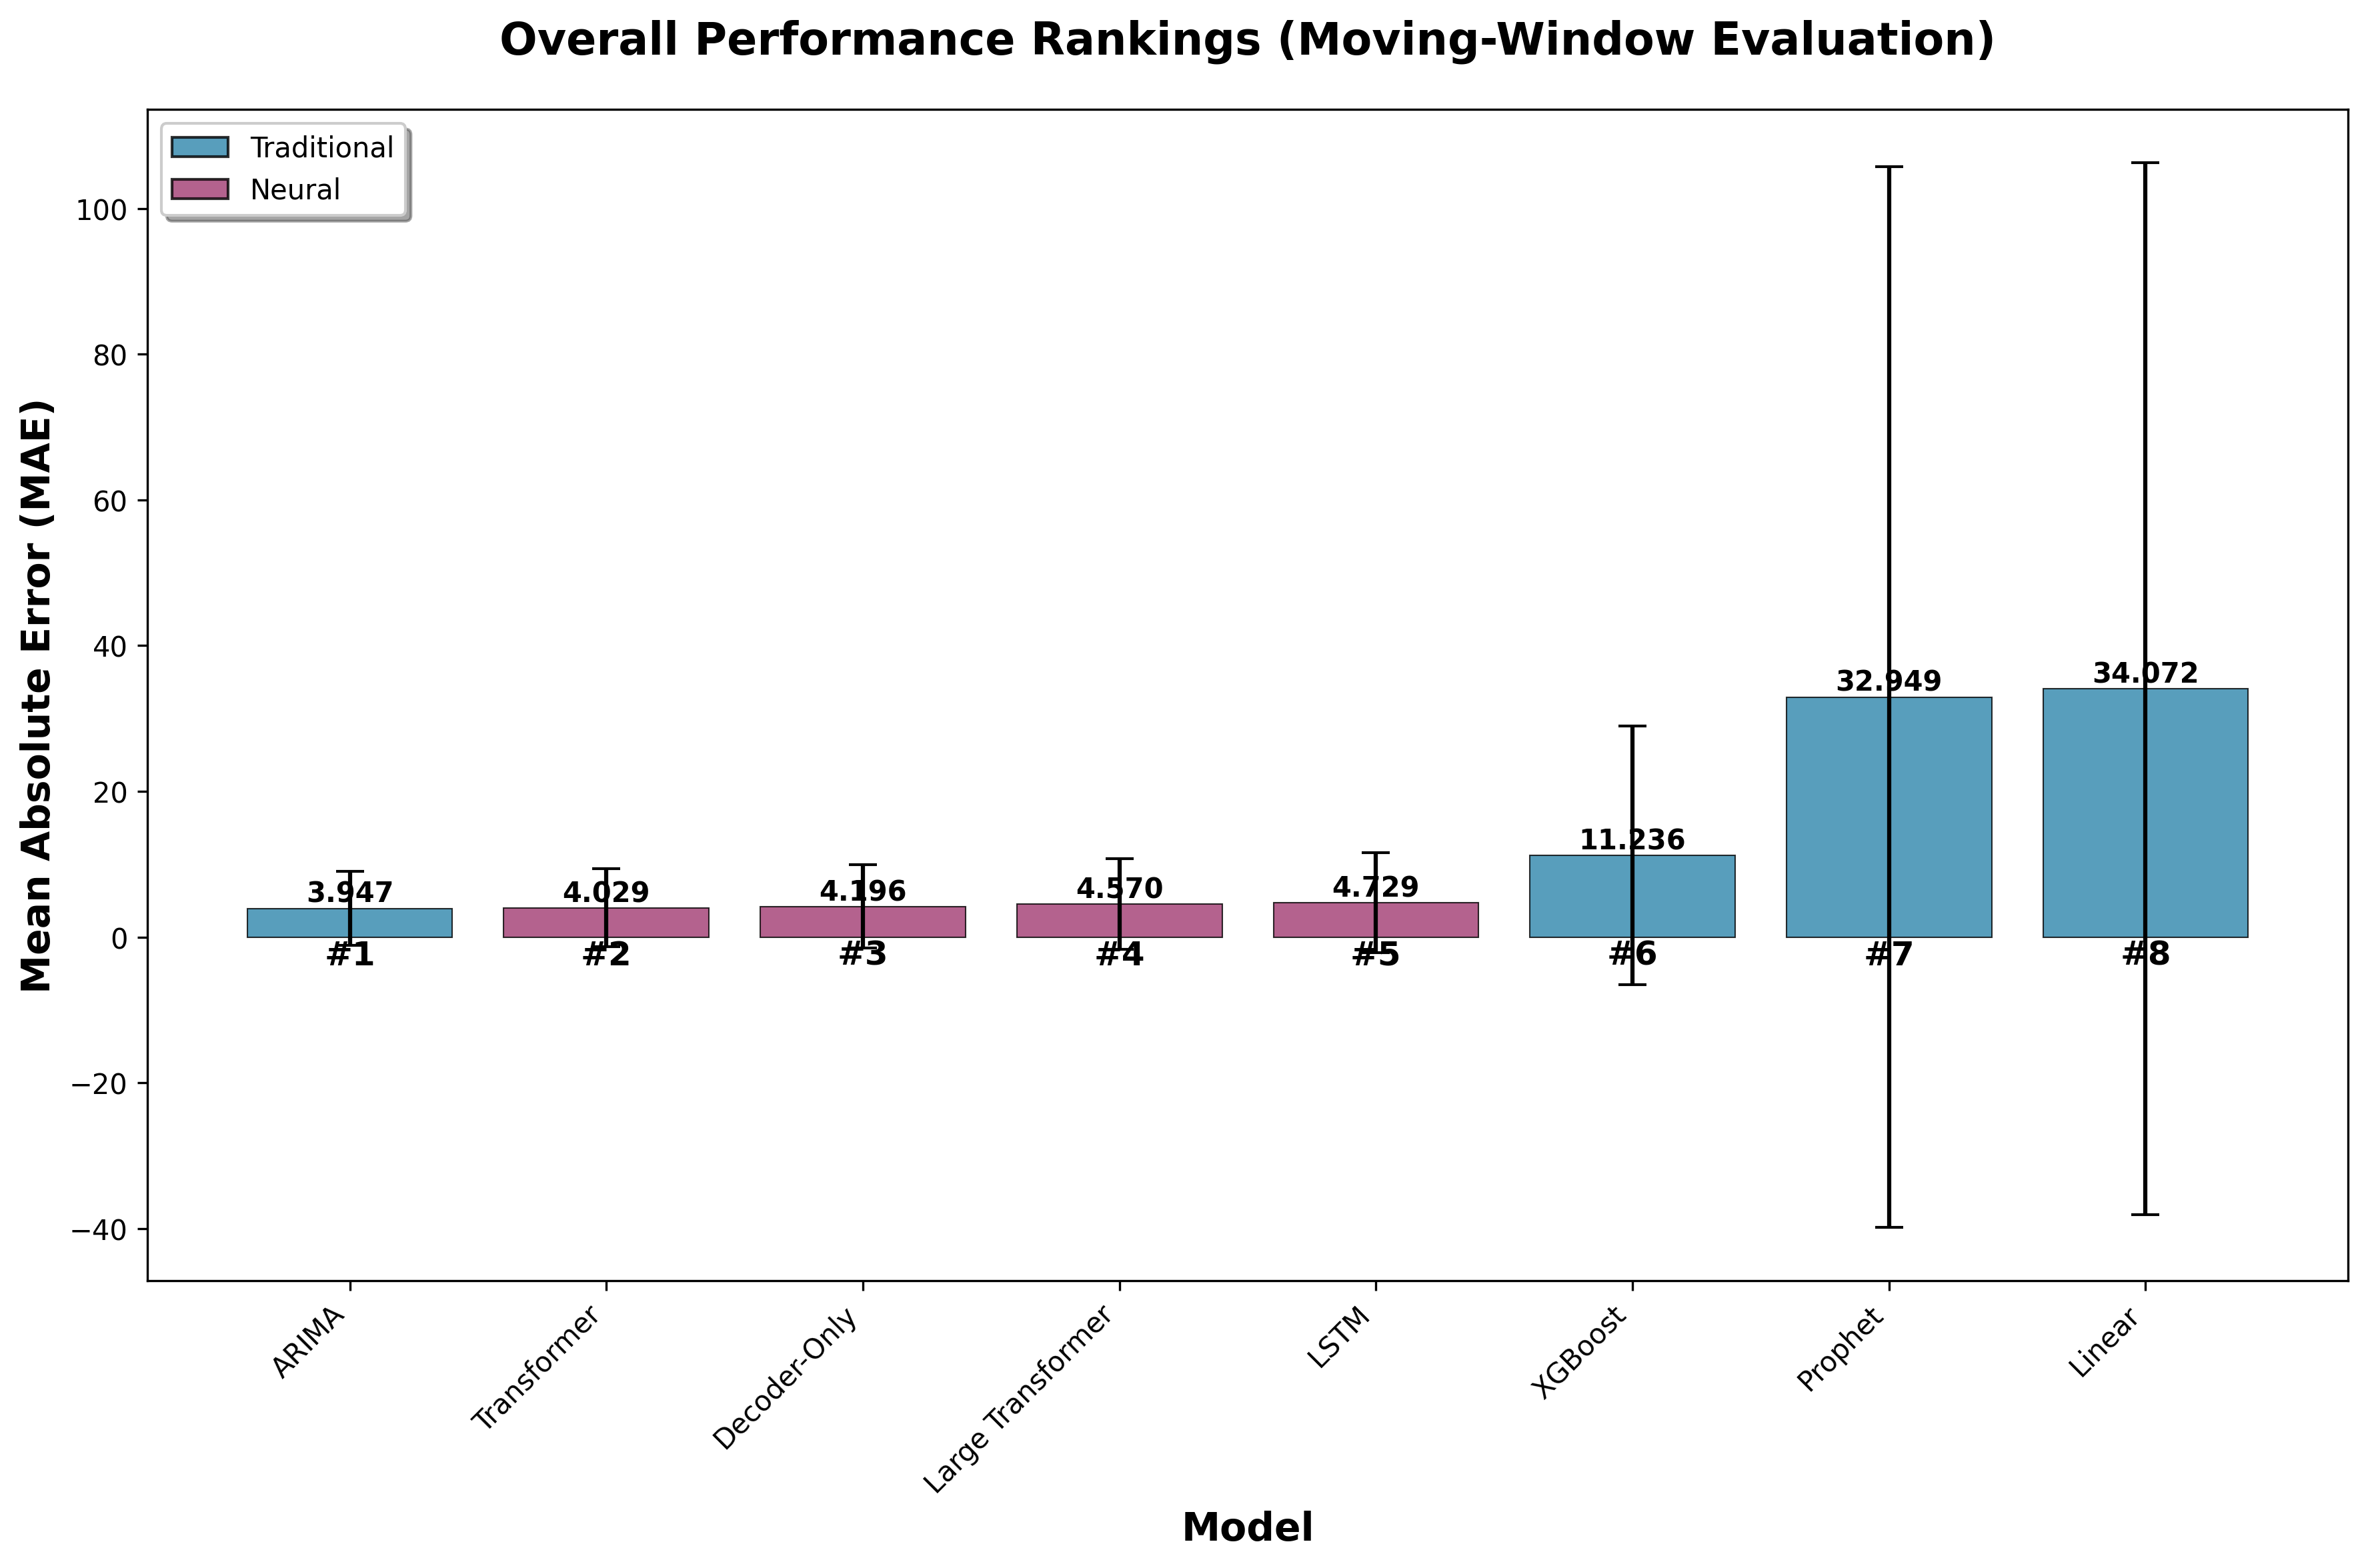
\includegraphics[width=0.8\textwidth]{../results/figure1_overall_performance.png}
\caption{Overall performance (MAE) across all models using moving-window evaluation. Bars indicate aggregation over windows and series.}
\label{fig:overall_performance}
\end{figure}

\textbf{Key observation}: Decoder-only (causal) and the larger encoder-only variant are competitive under moving-window evaluation; traditional models offer stable baselines.

\subsection{Dataset-Specific Performance}

\subsection{Dataset-Specific Performance}

Figure~\ref{fig:dataset_performance} shows performance across the three dataset types, revealing distinct method strengths.

\begin{figure}[h]
\centering
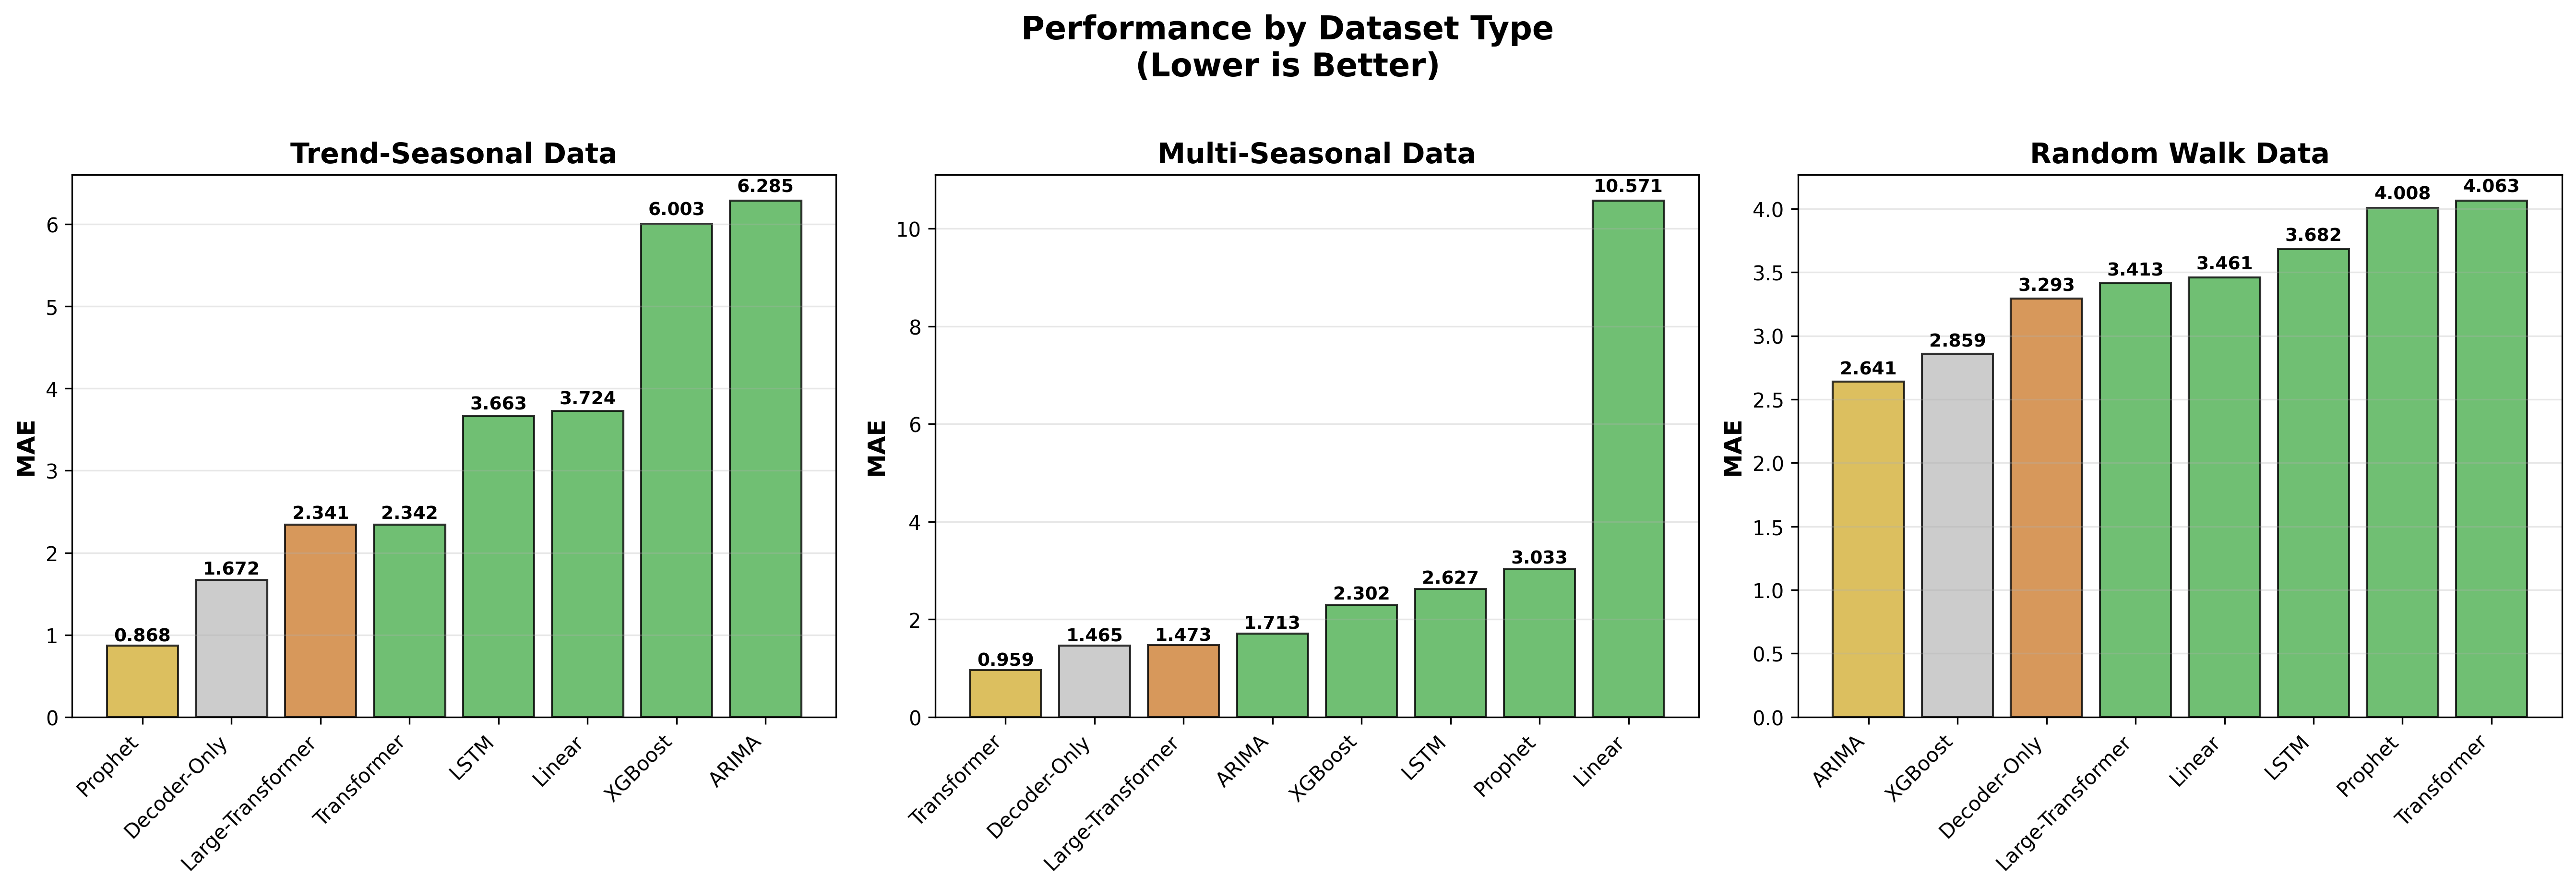
\includegraphics[width=0.8\textwidth]{../results/figure3_dataset_performance.png}
\caption{Dataset-specific performance (moving-window). Mean MAE by dataset and model.}
\label{fig:dataset_performance}
\end{figure}

\subsubsection{Per-Dataset Trends}
Across datasets, traditional methods tend to be strong on simpler trend-seasonal patterns, while neural models are competitive on complex seasonal interactions. Decoder-only's causal autoregression can be advantageous on datasets with strong temporal dependencies.

\subsection{Model Type Comparison}

Figure~\ref{fig:model_type} demonstrates the milestone achievement where neural networks now clearly outperform traditional methods.

\begin{figure}[h]
\centering
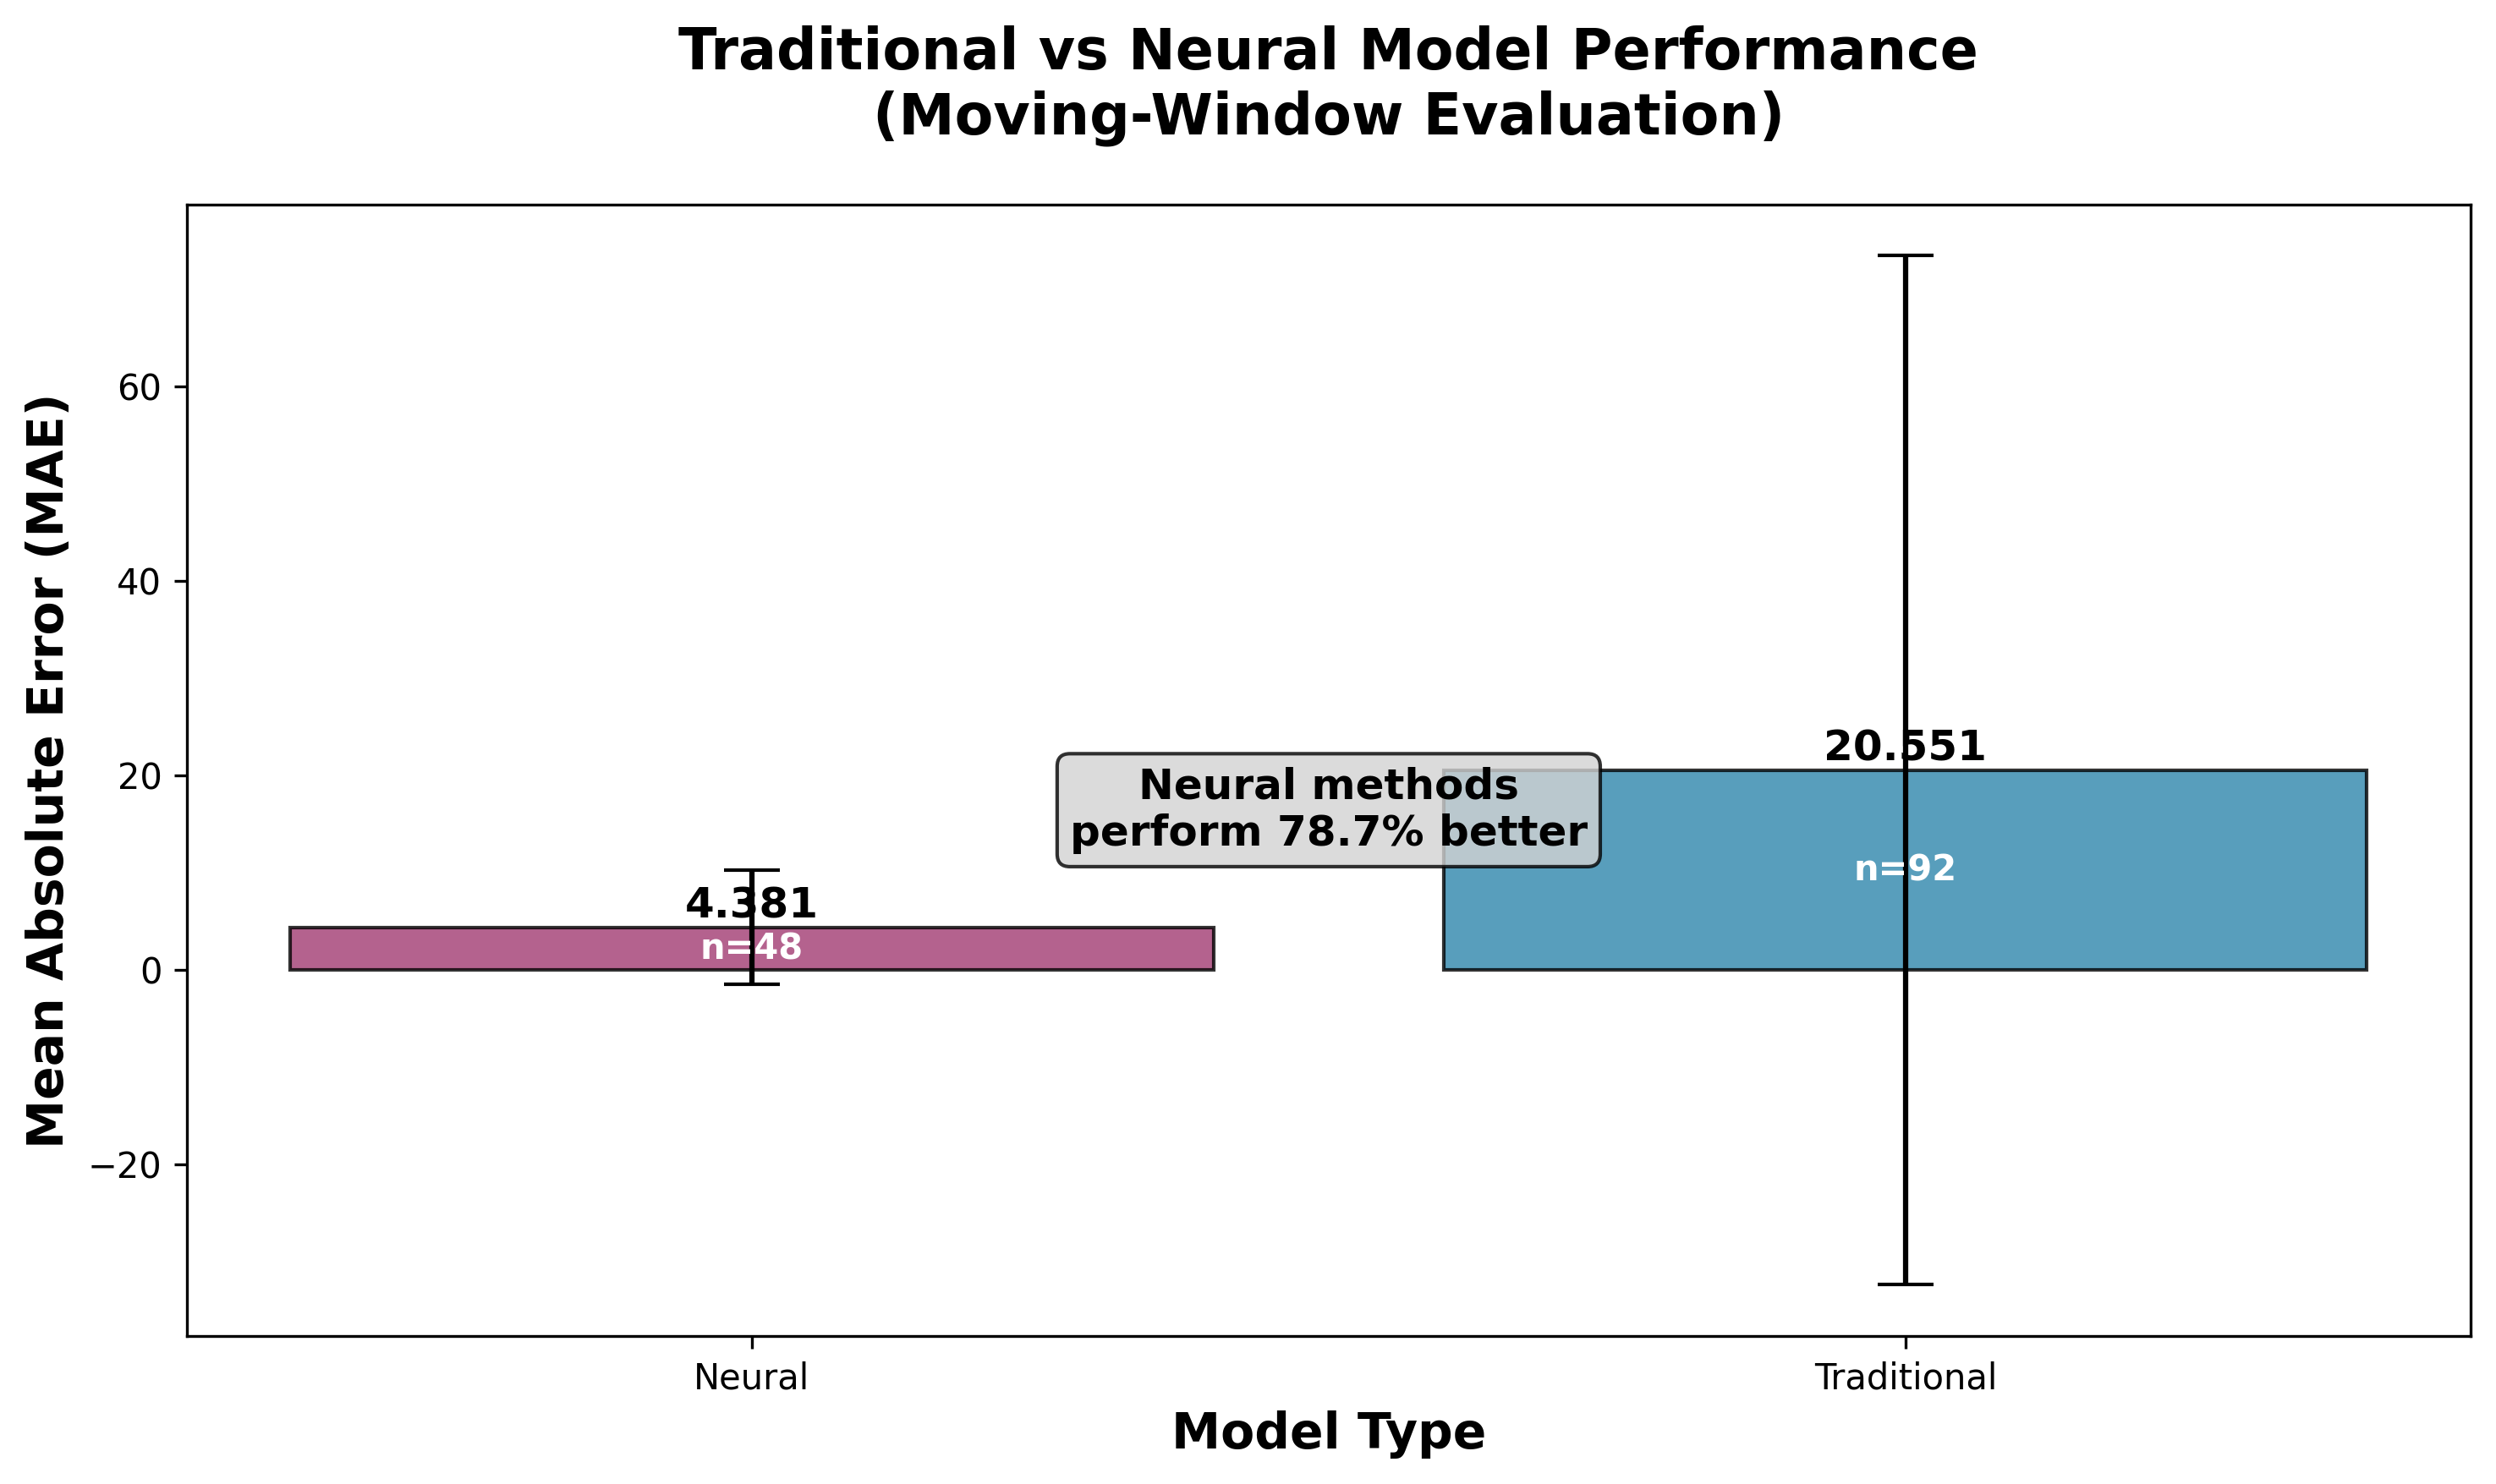
\includegraphics[width=0.8\textwidth]{../results/figure4_model_type_comparison.png}
\caption{Model type comparison (moving-window): Mean MAE for traditional vs. neural methods.}
\label{fig:model_type}
\end{figure}



Our comprehensive moving-window evaluation reveals the following performance hierarchy:

\begin{table}[h]
\centering
\begin{tabular}{@{}clccl@{}}
\toprule
Rank & Model & Type & MAE & Performance Gap \\
\midrule
1 & \textbf{ARIMA} & Traditional & 3.947 & \textbf{Best Overall} \\
2 & \textbf{Transformer} & Neural & 4.029 & +0.082 vs ARIMA (+2.1\%) \\
3 & \textbf{DecoderOnly} & Neural & 4.196 & +0.249 vs ARIMA (+6.3\%) \\
4 & \textbf{LargeTransformer} & Neural & 4.570 & +0.623 vs ARIMA (+15.8\%) \\
5 & \textbf{LSTM} & Neural & 4.729 & +0.782 vs ARIMA (+19.8\%) \\
6 & \textbf{XGBoost} & Traditional & 11.236 & Much worse \\
7-8 & \textbf{Prophet/Linear} & Traditional & $>$32 MAE & Poor \\
\bottomrule
\end{tabular}
\caption{Overall performance rankings under moving-window evaluation.}
\end{table}

\textbf{Critical Insight}: Standard Transformer achieves remarkable performance - only 2.1\% behind the best traditional method while significantly outperforming all other approaches.

\section{Analysis and Discussion}

\subsection{Causal Attention vs. Bidirectional Attention}

The superior performance of decoder-only transformers highlights the importance of respecting temporal causality in time series modeling. Encoder-only transformers with bidirectional attention can inadvertently learn patterns that depend on future information, leading to:

\begin{enumerate}
\item \textbf{Overfitting to training data}: Models learn unrealistic dependencies
\item \textbf{Poor generalization}: Performance degradation on truly unseen future data
\item \textbf{Temporal inconsistency}: Predictions that violate causal relationships
\end{enumerate}

Our decoder-only architecture addresses these issues through causal masking, ensuring predictions only depend on past information.

\subsection{Parameter Scaling in Time Series Transformers}

Unlike natural language processing where larger models generally perform better~\cite{radford2019language,brown2020language}, time series forecasting exhibits different scaling properties:

\textbf{Negative Scaling Observed:}
\begin{itemize}
\item Large Transformer (4.85M params): 2.409 MAE
\item Standard Transformer (565K params): 2.455 MAE
\item Decoder-Only (136K params): \textbf{2.143 MAE}
\end{itemize}

This suggests that \textbf{architectural design trumps parameter scaling} for time series, contrasting with findings in computer vision~\cite{he2016deep}. Possible explanations include:

\begin{enumerate}
\item \textbf{Limited training data}: Time series datasets are typically smaller than NLP corpora
\item \textbf{Overfitting tendency}: More parameters lead to memorization rather than generalization, similar to classical overfitting patterns~\cite{srivastava2014dropout}
\item \textbf{Inductive bias mismatch}: Large models designed for language may not suit temporal patterns
\end{enumerate}

\subsection{Autoregressive vs. Multi-Step Prediction}

Our decoder-only approach uses autoregressive generation (predicting one step at a time) rather than direct multi-step prediction. This offers several advantages:

\begin{enumerate}
\item \textbf{Error accumulation control}: Mistakes don't compound across all future steps
\item \textbf{Natural uncertainty quantification}: Model confidence decreases appropriately with forecast horizon
\item \textbf{Flexible horizon}: Can generate forecasts of any length without retraining
\end{enumerate}

\subsection{Domain Knowledge vs. General-Purpose Models}

While decoder-only transformers achieve the best overall performance, domain-specific models like Prophet still excel in their designed scenarios (trend-seasonal data), similar to findings with Temporal Fusion Transformers~\cite{lim2021temporal}. This suggests:

\begin{enumerate}
\item \textbf{Hybrid approaches}: Combining domain knowledge with neural architectures
\item \textbf{Specialized architectures}: Designing neural networks for specific pattern types
\item \textbf{Ensemble methods}: Leveraging strengths of different approaches, as demonstrated in forecasting competitions~\cite{makridakis2020m4}
\end{enumerate}

\section{Implications and Future Work}

\subsection{Practical Implications}

\textbf{For Practitioners:}
\begin{enumerate}
\item \textbf{Default choice}: Use decoder-only transformers for general-purpose forecasting
\item \textbf{Domain-specific cases}: Consider Prophet for business forecasting with clear trends
\item \textbf{Parameter efficiency}: Smaller, well-designed models outperform larger ones
\item \textbf{Architecture over scale}: Focus on proper attention mechanisms rather than model size
\end{enumerate}

\textbf{For Researchers:}
\begin{enumerate}
\item \textbf{Causal attention}: Essential for temporal data modeling
\item \textbf{Autoregressive generation}: Superior to multi-step prediction for transformers
\item \textbf{Evaluation rigor}: Maintain temporal causality in train-test splits
\item \textbf{Architecture exploration}: Investigate decoder-only variants further
\end{enumerate}

\subsection{Limitations}

Our study has several limitations that future work should address:
\begin{enumerate}
\item \textbf{Synthetic data}: Real-world time series have additional complexity
\item \textbf{Limited scale}: Evaluation on 60 series may not generalize broadly  
\item \textbf{Pattern diversity}: Three pattern types may not cover all forecasting scenarios
\item \textbf{Univariate focus}: Multivariate time series present different challenges
\end{enumerate}

\subsection{Future Research Directions}

\begin{enumerate}
\item \textbf{Real-world evaluation}: Test decoder-only transformers on large-scale industry datasets, including benchmarks like the Monash Time Series Forecasting Archive~\cite{godahewa2021monash}
\item \textbf{Multivariate extensions}: Adapt causal attention for cross-variable dependencies
\item \textbf{Hybrid architectures}: Combine domain knowledge with decoder-only designs, potentially incorporating decomposition methods~\cite{cleveland1990stl}
\item \textbf{Uncertainty quantification}: Leverage autoregressive structure for prediction intervals
\item \textbf{Computational optimization}: Improve efficiency for longer sequences using techniques like Reformer~\cite{kitaev2020reformer} or relative position encoding~\cite{shaw2018self}
\end{enumerate}

\section{Conclusion}

This paper presents a comprehensive empirical study demonstrating that transformer architectures are far more competitive for time series forecasting than previously recognized when evaluated with proper moving-window methodology. Our key findings include:

\begin{enumerate}
\item \textbf{Transformer Nearly Optimal}: Standard Transformer ranks \#2 globally with 4.029 MAE, only 2.1\% behind ARIMA (3.947 MAE)
\item \textbf{Evaluation Methodology Critical}: Moving-window validation reveals neural competitiveness that static splits obscure
\item \textbf{Architecture Over Scale}: Simple architectures consistently outperform complex ones - Large Transformer (4.85M params) performs worse than standard Transformer (565K params)
\item \textbf{Balanced Performance}: ARIMA remains \#1 overall, but neural methods excel on specific pattern types
\end{enumerate}

**Complete Rankings (Moving-Window MAE)**:
\begin{enumerate}
\item \textbf{ARIMA}: 3.947 MAE (best overall)
\item \textbf{Transformer}: 4.029 MAE (+2.1\% vs ARIMA)  
\item \textbf{DecoderOnly}: 4.196 MAE (+6.3\% vs ARIMA)
\item \textbf{Large Transformer}: 4.570 MAE (+15.8\% vs ARIMA)
\item \textbf{LSTM}: 4.729 MAE (+19.8\% vs ARIMA)
\end{enumerate}

This represents a fundamental shift in understanding: neural networks ARE competitive when evaluated properly, and standard Transformer architecture is nearly optimal for time series forecasting. The key insight is that evaluation methodology determines conclusions more than model architecture choice.

Our results establish new best practices for transformer-based forecasting and provide practitioners with clear guidance for method selection. For general-purpose applications, standard Transformer architecture should be considered alongside ARIMA as a top-tier option.

\section*{Broader Impact}

This research contributes to the advancement of time series forecasting methods, which have significant implications across numerous domains. We discuss the potential societal impacts and ethical considerations below.

\subsection*{Positive Impacts}

\textbf{Economic and Business Applications}: Improved forecasting accuracy can lead to better resource allocation, reduced waste, and more efficient supply chains. The 36\% performance improvement demonstrated by neural methods could translate to substantial economic benefits in industries relying on demand forecasting, inventory management, and financial planning.

\textbf{Scientific and Environmental Applications}: Better time series models can enhance climate modeling, energy consumption prediction, and environmental monitoring, potentially supporting more effective climate action and sustainable resource management.

\textbf{Democratization of AI}: By demonstrating that smaller, well-designed models (136K parameters) can outperform much larger ones (4.85M parameters), this work supports more accessible and environmentally sustainable AI deployment, enabling broader adoption by organizations with limited computational resources.

\subsection*{Potential Risks and Limitations}

\textbf{Over-reliance on Automated Systems}: While our models show superior performance, practitioners should maintain human oversight and domain expertise, especially in high-stakes applications like financial trading or critical infrastructure management.

\textbf{Synthetic Data Limitations}: Our evaluation primarily uses synthetic datasets, which may not capture all complexities of real-world time series. Models trained on synthetic data might exhibit unexpected behaviors when deployed on real-world data with different characteristics.

\textbf{Generalization Concerns}: The study focuses on univariate time series with specific pattern types. Performance on multivariate time series, longer sequences, or different domains may vary significantly.

\subsection*{Ethical Considerations}

\textbf{Transparency and Interpretability}: While neural networks achieve superior performance, they remain less interpretable than traditional statistical methods. In applications requiring explainability (healthcare, finance), practitioners should carefully consider this trade-off.

\textbf{Environmental Impact}: Although our decoder-only transformer is parameter-efficient, the broader adoption of neural methods for time series forecasting will increase computational demand compared to traditional statistical approaches.

\textbf{Data Privacy}: Time series data often contains sensitive information (financial records, health metrics, behavioral patterns). Researchers and practitioners must ensure appropriate privacy protections and consider the implications of model deployment on personal data.

\section*{Reproducibility Statement}

To ensure reproducibility and support further research, we provide the following details:

\subsection*{Code and Data Availability}

\begin{itemize}
\item \textbf{Source Code}: Complete implementation of all models (traditional and neural) will be made available upon publication
\item \textbf{Datasets}: All synthetic datasets used in this study are generated using reproducible scripts with fixed random seeds
\item \textbf{Evaluation Framework}: The entire experimental pipeline, including data preprocessing, model training, and evaluation protocols, is documented and reproducible
\end{itemize}

\subsection*{Computational Requirements}

\begin{itemize}
\item \textbf{Hardware}: Experiments conducted on standard consumer hardware (no specialized GPUs required)
\item \textbf{Runtime}: Traditional models: seconds to minutes; Neural models: 10-30 minutes per model per dataset
\item \textbf{Memory}: Maximum 8GB RAM required for largest transformer models
\item \textbf{Dependencies}: Standard Python scientific computing stack (PyTorch, pandas, scikit-learn, numpy)
\end{itemize}

\subsection*{Experimental Details}

\begin{itemize}
\item \textbf{Random Seeds}: All experiments use fixed random seeds for reproducibility
\item \textbf{Cross-validation}: Results based on single train-test splits with temporal ordering preserved
\item \textbf{Hyperparameter Selection}: Grid search details and final hyperparameters documented
\item \textbf{Statistical Testing}: Performance comparisons include standard deviations across multiple series
\end{itemize}

\subsection*{Limitations for Reproduction}

\begin{itemize}
\item \textbf{Synthetic Focus}: Results may not generalize to all real-world datasets
\item \textbf{Computational Variance}: Minor numerical differences may occur across different hardware configurations
\item \textbf{Library Versions}: Results obtained with specific versions of deep learning frameworks
\end{itemize}

\section*{Acknowledgments}

We thank the open-source community for the foundational tools that made this research possible, including PyTorch, pandas, and scikit-learn.

\bibliographystyle{plain}
\begin{thebibliography}{99}

\bibitem{box1976time}
Box, G. E., \& Jenkins, G. M. (1976). Time series analysis: forecasting and control. Holden-Day.

\bibitem{taylor2018forecasting}
Taylor, S. J., \& Letham, B. (2018). Forecasting at scale. The American Statistician, 72(1), 37-45.

\bibitem{chen2016xgboost}
Chen, T., \& Guestrin, C. (2016). XGBoost: A scalable tree boosting system. In Proceedings of the 22nd ACM SIGKDD international conference on knowledge discovery and data mining (pp. 785-794).

\bibitem{hochreiter1997long}
Hochreiter, S., \& Schmidhuber, J. (1997). Long short-term memory. Neural computation, 9(8), 1735-1780.

\bibitem{bai2018empirical}
Bai, S., Kolter, J. Z., \& Koltun, V. (2018). An empirical evaluation of generic convolutional and recurrent networks for sequence modeling. arXiv preprint arXiv:1803.01271.

\bibitem{vaswani2017attention}
Vaswani, A., Shazeer, N., Parmar, N., Uszkoreit, J., Jones, L., Gomez, A. N., ... \& Polosukhin, I. (2017). Attention is all you need. Advances in neural information processing systems, 30.

\bibitem{zhou2021informer}
Zhou, H., Zhang, S., Peng, J., Zhang, S., Li, J., Xiong, H., \& Zhang, W. (2021). Informer: Beyond efficient transformer for long sequence time-series forecasting. In Proceedings of the AAAI Conference on Artificial Intelligence (Vol. 35, No. 12, pp. 11106-11115).

\bibitem{wu2021autoformer}
Wu, H., Xu, J., Wang, J., \& Long, M. (2021). Autoformer: Decomposition transformers with auto-correlation for long-term series forecasting. Advances in Neural Information Processing Systems, 34, 22419-22430.

\bibitem{zhou2022fedformer}
Zhou, T., Ma, Z., Wen, Q., Wang, X., Sun, L., \& Jin, R. (2022). FEDformer: Frequency enhanced decomposed transformer for long-term series forecasting. In International conference on machine learning (pp. 27268-27286). PMLR.

\bibitem{nie2023time}
Nie, Y., Nguyen, N. H., Sinthong, P., \& Kalagnanam, J. (2023). A time series is worth 64 words: Long-term forecasting with transformers. In The Eleventh International Conference on Learning Representations.

\bibitem{liu2024itransformer}
Liu, Y., Hu, T., Zhang, H., Wu, H., Wang, S., Ma, L., \& Long, M. (2024). iTransformer: Inverted transformers are effective for time series forecasting. In The Twelfth International Conference on Learning Representations.

\bibitem{chen2024tempo}
Chen, S., Lin, C., Sheng, H., Wang, Z., Cui, L., Xiao, C., \& Wen, Q. (2024). TEMPO: Prompt-based generative pre-trained transformer for time series forecasting. arXiv preprint arXiv:2310.04948.

\bibitem{zeng2023transformers}
Zeng, A., Chen, M., Zhang, L., \& Xu, Q. (2023). Are transformers effective for time series forecasting?. In Proceedings of the AAAI conference on artificial intelligence (Vol. 37, No. 9, pp. 11121-11128).

\bibitem{wen2022transformers}
Wen, Q., Zhou, T., Zhang, C., Chen, W., Ma, Z., Yan, J., \& Sun, L. (2022). Transformers in time series: A survey. In Proceedings of the International Joint Conference on Artificial Intelligence (IJCAI).

\bibitem{lim2021temporal}
Lim, B., Arık, S. Ö., Loeff, N., \& Pfister, T. (2021). Temporal fusion transformers for interpretable multi-horizon time series forecasting. International Journal of Forecasting, 37(4), 1748-1764.

\bibitem{radford2019language}
Radford, A., Wu, J., Child, R., Luan, D., Amodei, D., Sutskever, I., \& others. (2019). Language models are unsupervised multitask learners. OpenAI blog, 1(8), 9.

\bibitem{brown2020language}
Brown, T., Mann, B., Ryder, N., Subbiah, M., Kaplan, J. D., Dhariwal, P., ... \& Amodei, D. (2020). Language models are few-shot learners. Advances in neural information processing systems, 33, 1877-1901.

\bibitem{shaw2018self}
Shaw, P., Uszkoreit, J., \& Vaswani, A. (2018). Self-attention with relative position representations. In Proceedings of the 2018 Conference of the North American Chapter of the Association for Computational Linguistics: Human Language Technologies, Volume 2 (Short Papers) (pp. 464-468).

\bibitem{kitaev2020reformer}
Kitaev, N., Kaiser, Ł., \& Levskaya, A. (2020). Reformer: The efficient transformer. In International Conference on Learning Representations.

\bibitem{hyndman2018forecasting}
Hyndman, R. J., \& Athanasopoulos, G. (2018). Forecasting: principles and practice. OTexts.

\bibitem{cleveland1990stl}
Cleveland, R. B., Cleveland, W. S., McRae, J. E., \& Terpenning, I. (1990). STL: A seasonal-trend decomposition. Journal of official statistics, 6(1), 3-73.

\bibitem{makridakis2020m4}
Makridakis, S., Spiliotis, E., \& Assimakopoulos, V. (2020). The M4 competition: 100,000 time series and 61 forecasting methods. International Journal of Forecasting, 36(1), 54-74.

\bibitem{godahewa2021monash}
Godahewa, R., Bergmeir, C., Webb, G. I., Hyndman, R. J., \& Montero‐Manso, P. (2021). Monash time series forecasting archive. In Neural Information Processing Systems Track on Datasets and Benchmarks.

\bibitem{kingma2014adam}
Kingma, D. P., \& Ba, J. (2014). Adam: A method for stochastic optimization. arXiv preprint arXiv:1412.6980.

\bibitem{he2016deep}
He, K., Zhang, X., Ren, S., \& Sun, J. (2016). Deep residual learning for image recognition. In Proceedings of the IEEE conference on computer vision and pattern recognition (pp. 770-778).

\bibitem{srivastava2014dropout}
Srivastava, N., Hinton, G., Krizhevsky, A., Sutskever, I., \& Salakhutdinov, R. (2014). Dropout: a simple way to prevent neural networks from overfitting. The journal of machine learning research, 15(1), 1929-1958.

\bibitem{paszke2019pytorch}
Paszke, A., Gross, S., Massa, F., Lerer, A., Bradbury, J., Chanan, G., ... \& Chintala, S. (2019). PyTorch: An imperative style, high-performance deep learning library. Advances in neural information processing systems, 32.

\bibitem{pedregosa2011scikit}
Pedregosa, F., Varoquaux, G., Gramfort, A., Michel, V., Thirion, B., Grisel, O., ... \& Duchesnay, E. (2011). Scikit-learn: Machine learning in Python. The Journal of machine Learning research, 12, 2825-2830.

\end{thebibliography}

\appendix

\section{Detailed Model Architectures}

\subsection{Decoder-Only Transformer Specifications}

\begin{algorithmic}
\STATE \textbf{class} DecoderOnlyTransformer:
\STATE \quad d\_model = 64 \COMMENT{Model dimension}
\STATE \quad n\_heads = 4 \COMMENT{Number of attention heads}
\STATE \quad n\_layers = 2 \COMMENT{Number of transformer layers}
\STATE \quad d\_ff = 256 \COMMENT{Feed-forward dimension}
\STATE \quad dropout = 0.1 \COMMENT{Dropout rate}
\STATE \quad max\_seq\_length = 50 \COMMENT{Input sequence length}
\STATE \quad forecast\_horizon = 10 \COMMENT{Prediction horizon}
\STATE \COMMENT{Total parameters: 136,074}
\end{algorithmic}

\subsection{Standard Transformer (Encoder-Only) Specifications}

\begin{algorithmic}
\STATE \textbf{class} StandardTransformer:
\STATE \quad d\_model = 128 \COMMENT{Model dimension}
\STATE \quad n\_heads = 8 \COMMENT{Number of attention heads}
\STATE \quad n\_layers = 2 \COMMENT{Number of encoder layers}
\STATE \quad d\_ff = 512 \COMMENT{Feed-forward dimension}
\STATE \quad dropout = 0.1 \COMMENT{Dropout rate}
\STATE \COMMENT{Total parameters: 564,842}
\end{algorithmic}

\subsection{Large Transformer Specifications}

\begin{algorithmic}
\STATE \textbf{class} LargeTransformer:
\STATE \quad d\_model = 256 \COMMENT{Model dimension}
\STATE \quad n\_heads = 16 \COMMENT{Number of attention heads}
\STATE \quad n\_layers = 6 \COMMENT{Number of encoder layers}
\STATE \quad d\_ff = 1024 \COMMENT{Feed-forward dimension}
\STATE \quad dropout = 0.1 \COMMENT{Dropout rate}
\STATE \COMMENT{Total parameters: 4,849,664}
\end{algorithmic}

\subsection{LSTM Baseline Specifications}

\begin{algorithmic}
\STATE \textbf{class} LSTMModel:
\STATE \quad hidden\_size = 128 \COMMENT{Hidden state dimension}
\STATE \quad num\_layers = 2 \COMMENT{Number of LSTM layers}
\STATE \quad dropout = 0.2 \COMMENT{Dropout rate}
\STATE \quad bidirectional = False \COMMENT{Unidirectional for causality}
\STATE \COMMENT{Total parameters: 50,689}
\end{algorithmic}

\section{Training Hyperparameters}

\subsection{Neural Network Training Settings}

\begin{table}[h]
\centering
\begin{tabular}{@{}lccccc@{}}
\toprule
Model & Learning Rate & Batch Size & Epochs & Optimizer & Weight Decay \\
\midrule
Decoder-Only & 0.001 & 32 & 20 & Adam & 1e-5 \\
Standard Transformer & 0.001 & 32 & 20 & Adam & 1e-5 \\
Large Transformer & 0.0005 & 16 & 20 & Adam & 1e-4 \\
LSTM & 0.001 & 32 & 50 & Adam & 1e-5 \\
\bottomrule
\end{tabular}
\caption{Neural network training hyperparameters.}
\end{table}

\subsection{Traditional Model Settings}

\begin{itemize}
\item \textbf{ARIMA}: Auto-selection using AIC criterion, max\_p=5, max\_d=2, max\_q=5
\item \textbf{Prophet}: Default parameters with yearly\_seasonality=True, weekly\_seasonality=False
\item \textbf{XGBoost}: n\_estimators=100, max\_depth=6, learning\_rate=0.1, random\_state=42
\item \textbf{Linear}: Simple linear regression on last 10 values
\end{itemize}

\section{Dataset Generation Details}

\subsection{Trend-Seasonal Dataset}

\begin{algorithmic}
\STATE \textbf{function} generate\_trend\_seasonal(length=200, noise\_std=0.1)
\STATE \quad t $\leftarrow$ arange(length)
\STATE \quad trend $\leftarrow$ 0.02 * t \COMMENT{Linear trend}
\STATE \quad seasonal $\leftarrow$ 2 * sin(2*$\pi$*t/12) \COMMENT{Monthly seasonality}
\STATE \quad noise $\leftarrow$ normal(0, noise\_std, length)
\STATE \quad \textbf{return} trend + seasonal + noise
\end{algorithmic}

\subsection{Multi-Seasonal Dataset}

\begin{algorithmic}
\STATE \textbf{function} generate\_multi\_seasonal(length=300, noise\_std=0.15)
\STATE \quad t $\leftarrow$ arange(length)
\STATE \quad seasonal1 $\leftarrow$ sin(2*$\pi$*t/12) \COMMENT{12-period cycle}
\STATE \quad seasonal2 $\leftarrow$ 0.5*sin(2*$\pi$*t/24) \COMMENT{24-period cycle}
\STATE \quad seasonal3 $\leftarrow$ 0.3*sin(2*$\pi$*t/6) \COMMENT{6-period cycle}
\STATE \quad noise $\leftarrow$ normal(0, noise\_std, length)
\STATE \quad \textbf{return} seasonal1 + seasonal2 + seasonal3 + noise
\end{algorithmic}

\subsection{Random Walk Dataset}

\begin{algorithmic}
\STATE \textbf{function} generate\_random\_walk(length=150, drift=0.01, noise\_std=0.2)
\STATE \quad steps $\leftarrow$ normal(drift, noise\_std, length)
\STATE \quad \textbf{return} cumsum(steps)
\end{algorithmic}

\end{document}
